\section{The limiting conditional distribution}
\label{sec:qsd}

When absorption is inevitable --- as it is for \(p<\tfrac12\) --- the unconditional process eventually sits at extinction. Before that happens, however, the law of the population \emph{conditional on not yet being extinct} may settle to a time-independent distribution. That limiting conditional law is the quasi-stationary, or Yaglom, distribution \cite{Yaglom1947,Athreya1972}. This section establishes its first two moments for the binary Galton--Watson process.

\subsection{Late-time survival probability}
\label{sec:lateS}

Everything follows from the decay of \(S_n\). For \(p<\tfrac12\), death is more likely than division at each step, \(S_n\to0\), and the quadratic term in
\begin{equation*}
S_{n+1} = 2pS_n - pS_n^2
\end{equation*}
becomes negligible relative to the linear term. The recursion is then well approximated by
\begin{equation}
\label{attenuated}
S_{n+1} \approx 2p\,S_n,
\end{equation}
and at late times
\begin{equation}
\label{lateS}
S_n \sim A(p)\,(2p)^n \qquad (n\to\infty),
\qquad
A(p) = \lim_{n\to\infty}\frac{S_n}{(2p)^n}.
\end{equation}
The constant \(A(p)\) accumulates the effect of the quadratic correction over the early generations, before the linear regime takes hold. The limit exists, is finite, and is strictly positive for \(p\in[0,\tfrac12)\); existence via an infinite product is proved in \cref{sec:product}, and \cref{sec:Abounds} places \(A(p)\) in \((0,\tfrac12]\).

\begin{remark}
Relation \cref{lateS} is an asymptotic equivalence, not an identity for each \(n\). One must not write \(\lim_n S_n = A(p)(2p)^n\): the right-hand side still depends on \(n\). What converges is the ratio \(S_n/(2p)^n\).
\end{remark}

\subsection{Mean}
\label{sec:condmean}

Decompose the expected size into extinct and surviving contributions:
\begin{equation*}
\mean{\zz_n}
= \pr{\zz_n = 0}\,\cancelto{0}{\mean{\zz_n\mid \zz_n = 0}}
+ \pr{\zz_n > 0}\,\mean{\zz_n \mid \zz_n > 0}.
\end{equation*}
The first term vanishes, so with \(\pr{\zz_n>0}=S_n\) and \(\mean{\zz_n}=(2p)^n\),
\begin{equation}
\label{eq:condmeandef}
\mean{\zz_n \mid \zz_n > 0} = \frac{\mean{\zz_n}}{S_n} = \frac{(2p)^n}{S_n}.
\end{equation}
Inserting \cref{lateS},
\begin{equation}
\label{eq:qsmean}
\mean{\zz_n \mid \zz_n > 0} \;\xrightarrow[n\to\infty]{}\; \frac{1}{A(p)}.
\end{equation}
The geometric factors cancel exactly. At late times the surviving population has constant expected size \(1/A(p)\), the \emph{quasi-stationary mean}.

\Cref{fig:condmean} shows the approach to the plateau. The closer \(p\) is to \(\tfrac12\), the higher the plateau and the longer the wait --- the near-critical difficulty that \cref{sec:Ap} must confront.

\begin{figure}[ht]
\centering
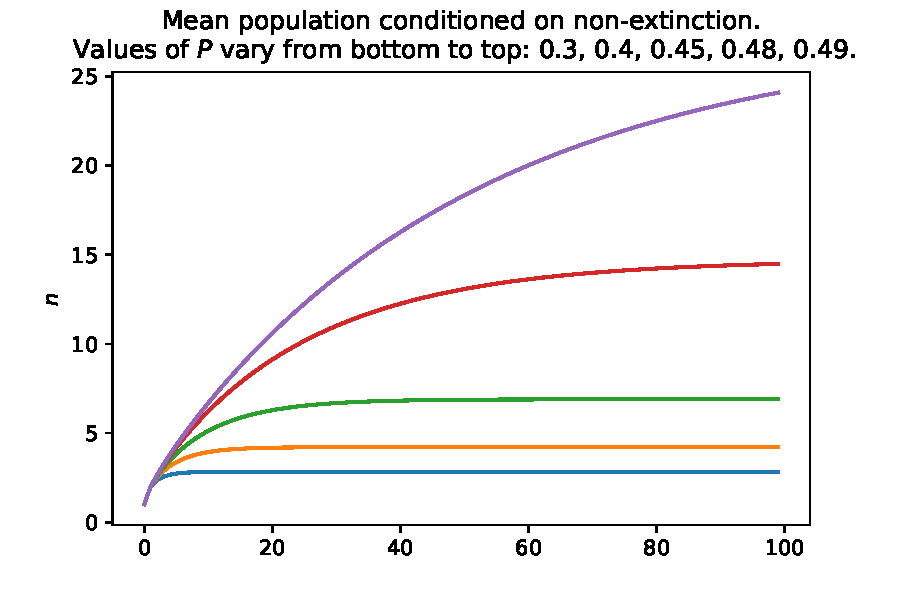
\includegraphics[width=0.78\textwidth]{figures/IMG_ch3/conditionalMean.pdf}
\caption{Conditional mean \((2p)^n/S_n\) against generation \(n\), with \(S_n\) from iterating \cref{SnIter}. From bottom to top, \(p = 0.3,\,0.4,\,0.45,\,0.48,\,0.49\). Each curve approaches \(1/A(p)\); approximate plateaus are \(2.825\), \(4.208\), \(6.893\), \(14.703\) and \(27.476\) (computed as in \cref{sec:practical}). Near \(p=0.49\) convergence is visibly slow.}
\label{fig:condmean}
\end{figure}

\subsection{Variance}
\label{sec:variance}

Stabilisation of the conditional mean is not enough for quasi-stationarity of the full law; the second moment is needed.

\subsubsection{The second moment \(\mean{\zz_n^2}\)}

For a random variable \(\xx\) the moment generating function is \(\mean{\ee^{t\xx}}\), which may be written through the \pgf{} as \(\phi(\ee^t)\). For the binary offspring law \cref{eq:pgfbinary},
\begin{equation}
\label{mgf1}
M_1(t) = \phi_1(\ee^t) = p\,\ee^{2t} + (1-p),
\end{equation}
the subscript \(1\) marking generation \(n=1\). Moments follow from
\begin{equation}
\label{mgf2}
\mean{\zz_n^r} = \frac{\dd^r}{\dd t^r}M_n(t)\bigg|_{t=0}.
\end{equation}
Differentiating \cref{mgf1} twice at \(t=0\) gives \(\mean{\zz_1^2}=4p\). To reach generation \(n\), recall that the \(n\)-step \pgf{} is the \(n\)-fold composition of \(\phi_1\), so
\begin{equation*}
M_n(t) = \phi_1\lrbq{\phi_1\lrbq{\dots\phi_1\lrbq{\ee^t}}}.
\end{equation*}
Differentiating once by the chain rule,
\begin{equation}
\label{dmgf1}
M_n'(t) = \phi_1'\lrbq{\phi_{n-1}\lrbq{\ee^t}}\cdot\phi_1'\lrbq{\phi_{n-2}\lrbq{\ee^t}}\cdots\phi_1'\lrbq{\ee^t}\cdot\ee^t .
\end{equation}
Since \(\phi_1'(z)=2pz\), this collapses to
\begin{equation}
\label{dmgf2}
M_n'(t) = (2p)^n\cdot M_{n-1}(t)\cdot M_{n-2}(t)\cdots M_1(t)\cdot\ee^{2t}.
\end{equation}
At \(t=0\) every factor equals \(1\). Differentiating the product \cref{dmgf2} produces a sum of terms in which exactly one factor is differentiated:
\begin{align*}
M_n''(t) = (2p)^n\bigg[\,&M_{n-1}'(t)\cdot M_{n-2}(t)\cdots M_1(t)\cdot\ee^{2t}\\
+ &M_{n-1}(t)\cdot M_{n-2}'(t)\cdots M_1(t)\cdot\ee^{2t}\\
&\hspace{60pt}\vdots\\
+ &M_{n-1}(t)\cdot M_{n-2}(t)\cdots M_1'(t)\cdot\ee^{2t}\\
+ &M_{n-1}(t)\cdot M_{n-2}(t)\cdots M_1(t)\cdot 2\ee^{2t}\,\bigg].
\end{align*}
Evaluating at \(t=0\) and using \(M_k'(0)=(2p)^k\) yields
\begin{equation*}
M_n''(0) = (2p)^n\lrbs{\sum_{i=0}^{n-1}(2p)^i + 1}.
\end{equation*}
Summing the geometric series and rearranging,
\begin{equation}
\label{secondMoment}
\mean{\zz_n^2} = (2p)^n\lrb{1 + \frac{1}{1-2p}} - (2p)^{2n}\lrb{\frac{1}{1-2p}},
\end{equation}
which recovers \(\mean{\zz_1^2}=4p\) at \(n=1\).

\subsubsection{Late-time variance}

From \(\mathrm{Var}(\zz_n)=\mean{\zz_n^2}-\mean{\zz_n}^2\) and \cref{secondMoment}, for \(2p<1\) the leading large-\(n\) term of the unconditional variance is of order \((2p)^n\). Conditional moments, however, are formed by dividing by \(S_n\). Using \cref{lateS},
\begin{align*}
\mean{\zz_n^2\mid \zz_n\neq0} &\xrightarrow{n\to\infty}
\frac{1}{A}\lrb{1+\frac{1}{1-2p}},\\[4pt]
\mean{\zz_n\mid \zz_n\neq0} &\xrightarrow{n\to\infty}
\frac{1}{A},
\end{align*}
so the conditional variance tends to a finite constant:
\begin{equation}
\label{eq:condvar}
\mathrm{Var}(\zz_n\mid \zz_n\neq0) \;\longrightarrow\; \frac{1}{A}\lrb{1+\frac{1}{1-2p}} - \frac{1}{A^2}.
\end{equation}
Both conditional moments are expressed entirely in terms of \(p\) and the single unknown \(A(p)\). Higher moments settle by the same mechanism, yielding the full quasi-stationary distribution. Everything now turns on that constant.

\subsection{A continuum view of the survival recursion}
\label{sec:riccati}

Write \(r=1-2p\) for the distance from criticality. The recursion \cref{SnIter} rearranges to
\begin{equation}
\label{eq:Sdiff}
S_{n+1}-S_n = -r S_n - p S_n^2 .
\end{equation}
For large \(n\) the left-hand side is well approximated by a derivative, giving the Riccati equation
\begin{equation}
\label{eq:riccati}
\frac{\dd S}{\dd n} = -r S - p S^2 .
\end{equation}
The substitution \(u=1/S\) linearises it to \(u'=ru+p\), with solution
\begin{equation}
\label{eq:riccatisol}
S(n) = \frac{r}{K r\,\ee^{rn} - p},
\end{equation}
\(K\) fixed by initial data. Setting \(r=0\) recovers the critical scaling \(S\sim2/n\); keeping \(r>0\) recovers geometric decay of the form \(S\sim A(2p)^n\). The integration constant \(K\) is determined by early generations where the continuum approximation fails --- which is another way of saying that it is \(A(p)\), and that no purely continuum argument will produce it. \Cref{sec:asymptotic} extracts what can still be obtained near criticality.

\FloatBarrier
